%!TEX program = xelatex
\documentclass[aspectratio=43,UTF8,10pt]{ctexbeamer}

    \mode<presentation> {
    \usetheme{Madrid}
    %\setbeamertemplate{footline} % To remove the footer line in all slides uncomment this line
    \setbeamertemplate{footline}[frame number] % To replace the footer line in all slides with a simple slide count uncomment this line
    \setbeamercolor{page number in head/foot}{fg=blue}
    \setbeamertemplate{navigation symbols}{} % To remove the navigation symbols from the bottom of all slides uncomment this line
    }
    \usepackage{indentfirst}
    \setlength{\parindent}{2em}
    \usepackage{listings}
    \lstset{language=C++, showstringspaces=false, basicstyle=\small}
    \usepackage{wrapfig}
    \usepackage{graphicx}
    \usepackage{animate}
    % \usepackage{fboxrule}
\definecolor{hanblue}{rgb}{0.27, 0.42, 0.81}
\definecolor{indiagreen}{rgb}{0.07, 0.53, 0.03}
\definecolor{indianred}{rgb}{0.8, 0.36, 0.36}
\definecolor{indianyellow}{rgb}{0.89, 0.66, 0.34}
\definecolor{babypink}{rgb}{0.96, 0.76, 0.76}
\definecolor{ao(english)}{rgb}{0.0, 0.5, 0.0}

    \definecolor{azure(colorwheel)}{rgb}{0.0, 0.5, 1.0}
    \definecolor{alizarin}{rgb}{0.82, 0.1, 0.26}
    % User Defined Block %%%%%%%%%%%%%%%%%%%%%%%%%%%%%%%%%%%%%%%%%%%%%%%%%%%%%%%%




    \newenvironment<>{blueblock}[1]{%
      \setbeamercolor{block title}{fg=white,bg=hanblue}%
    %   \setbeamercolor{block body}{fg=white,bg=bondiblue}%
      \begin{block}#2{#1}}{\end{block}}

    \newenvironment<>{greenblock}[1]{%
    % \setbeamercolor{block title}{fg=white,bg=bondiblue}%
      \setbeamercolor{block title}{fg=white,bg=indiagreen}%
    \begin{block}#2{#1}}{\end{block}}

    \newenvironment<>{redblock}[1]{%
      \setbeamercolor{block title}{fg=white,bg=indianred}%
    %   \setbeamercolor{block body}{fg=white,bg=bondiblue}%
      \begin{block}#2{#1}}{\end{block}}

    \newenvironment<>{yellowblock}[1]{%
      \setbeamercolor{block title}{fg=white,bg=indianyellow}%
      \begin{block}#2{#1}}{\end{block}}

    \lstset{language=C++,
    columns=flexible,
    basicstyle=\footnotesize\ttfamily,                                    % 设定代码字体、大小
    %numbers=left,xleftmargin=2em,framexleftmargin=2em,                   % 在左侧显示行号
    %numberstyle=\color{darkgray},                                        % 设定行号格式
    keywordstyle=\color{blue},                                            % 设定关键字格式
    commentstyle=\color{ao(english)},                                     % 设置代码注释的格式
    stringstyle=\color{brown},                                            % 设置字符串格式
    showstringspaces=false,                                              % 控制是否显示空格
    %frame=single,                                                         % 控制外框
    breaklines,                                                           % 控制是否折行
    % postbreak=\space,                                                     % 控制折行后显示的标识字符
    breakindent=5pt,                                                      % 控制折行后缩进数量
    emph={size\_t,array,deque,list,map,queue,set,stack,vector,string,pair,tuple,ostream}, % 非内置类型
    emphstyle={\color{teal}},
    escapeinside={(*@}{@*)},
}

\usepackage{multicol}

%----------------------------------------------------------------------------------------
%	TITLE PAGE
%----------------------------------------------------------------------------------------



\title[\textit{C++程序设计:第五章}]{第五章~函数} % The short title appears at the bottom of every slide, the full title is only on the title page

%\author[李长河]{李长河} % Your name
%\institute[CUG] % Your institution as it will appear on the bottom of every slide, may be shorthand to save space
%{
%中国地质大学(武汉)\\ % Your institution for the title page
%\medskip
%\textit{lichanghe@cug.edu.cn} % Your email address
%}
\date{} % Date, can be changed to a custom date

\begin{document}

%----------------------------------------------------------------------------------------
%	TIKZ FLOWCHART
%----------------------------------------------------------------------------------------
%\tikzstyle{startstop} = [rectangle, rounded corners, minimum width=2cm, minimum height=0.5cm, text centered, draw=black, fill=red!30, font=\tiny]
%\tikzstyle{io} = [trapezium, trapezium left angle=70, trapezium right angle=110, minimum width=0cm, minimum height=0cm, text centered, draw=black, fill=blue!30, font=\tiny]
%\tikzstyle{process} = [rectangle, minimum width=2.5cm, minimum height=1.5cm, text centered, draw=black, fill=orange!30, font=\tiny, text width=2cm]
%\tikzstyle{decision} = [diamond, minimum width=2.5cm, minimum height=2cm, text centered, draw=black, fill=green!30, font=\tiny, text width=1.8cm, aspect=1.1]

\begin{frame}
\titlepage % Print the title page as the first slide
\end{frame}


\begin{frame}{目录}
\begin{multicols}{2}
  \tableofcontents
\end{multicols}
%\tableofcontents
\end{frame}

%----------------------------------------------------------------------------------------
%	PRESENTATION SLIDES
%----------------------------------------------------------------------------------------

%--------------------

\begin{frame}[fragile]{~} % Table of contents slide, comment this block out to remove it

\begin{block}{学习目标}
\begin{enumerate}
\item 掌握函数的定义,以及常用的参数传递方式和值返回方式;
\item 理解函数调用机制及对象生命期的概念;
\item 能够根据需要编写具有一定实际用途的函数;
\item 掌握递归程序设计方法和多文件结构的使用;
\end{enumerate}
\end{block}

% ------功能模块说明,请注释掉-------
%\begin{columns}[t]
%\column{0.18\textwidth}
%\begin{block}{概念}
%\end{block}
%\column{0.18\textwidth}
%\begin{blueblock}{代码}
%\end{blueblock}
%\column{0.18\textwidth}
%\begin{yellowblock}{说明}
%\end{yellowblock}
%\column{0.18\textwidth}
%\begin{greenblock}{问题/答案}
%\end{greenblock}
%\column{0.18\textwidth}
%\begin{redblock}{注意}
%\end{redblock}
%\end{columns}
% ------功能模块说明,请注释掉-------

\end{frame}

%--------------------

%#####################################
\section{认识函数}

\begin{frame}
    {5.1 认识函数}
    \begin{block}{函数}
   具有名字的语句块。
   \begin{itemize}
     \item  通过调用函数的名字可以执行相应的代码块;
     \item  模块化程序设计的基础。
   \end{itemize}
    \end{block}
\end{frame}

\subsection{定义函数}
\begin{frame}[fragile]
    {5.1 认识函数\small{~---~定义函数}}
\begin{block}{函数四要素}

       \begin{itemize}
      \item 返回值类型(return type);
      \item 函数名(function name);
      \item 参数列表(parameter list);
      \item 函数体(function body)。
    \end{itemize}

\end{block}

    \begin{blueblock}<2->{\texttt{maximum}函数:返回两个整数中较大的数}
\vspace{-1.5mm}\begin{lstlisting}
int maximum(int a, int b) { //a和b为两个int类型(*@\alert{形参}@*)
     int c;                //用来保存结果
     c=a > b ? a : b;
     return c;              //返回结果
}

\end{lstlisting}\vspace{-1.5mm}
\end{blueblock}

\end{frame}




\subsection{调用函数}
\begin{frame}[fragile]
    {5.1 认识函数\small{~---~调用函数}}

\begin{columns}
\column{0.5\textwidth}

    \begin{blueblock}{调用maxnum函数}
\vspace{-1.5mm}\begin{lstlisting}[basicstyle=\small\ttfamily]
int maximum(int a, int b) {
     int c;
     c=a > b ? a : b;
     return c;
}
int main() {
    int x, y, z;
    cin >> x >> y;
    //调用函数maximum,x和y为(*@\alert{实参}@*)
    z = maximum(x, y);
    cout << "The maximum value is " << z << endl;
    return 0;
}
\end{lstlisting}\vspace{-1.5mm}
\end{blueblock}


\column{0.5\textwidth}
%        \begin{column}{0.4\textwidth}
函数调用过程(如下):

            \begin{figure}[ht]
                \centering
                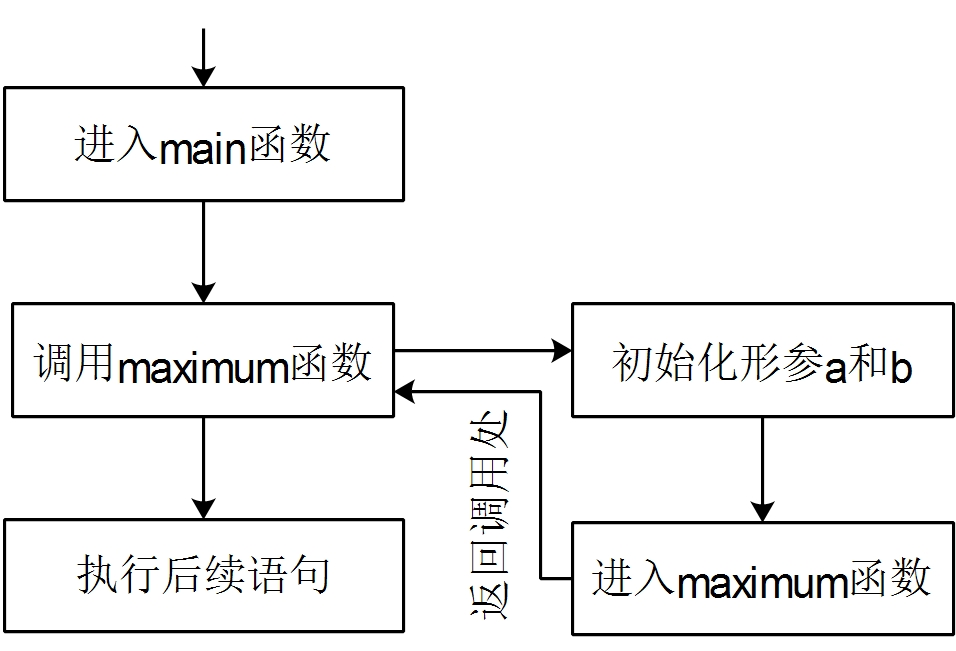
\includegraphics[scale=0.7]{Fig5-1}
                % \caption{\texttt{do while}语句执行流程}
                % \label{fig:label}
            \end{figure}
%\end{column}
\end{columns}

\end{frame}



\subsection{调用规则}

\begin{frame}[fragile]
    {5.1 认识函数\small{~---~调用规则}}
\begin{block}{调用规则}
\begin{itemize}
  \item 调用处的函数名要和被调函数的函数名一致;
  \item 实参和形参存在一一对应的关系,类型要兼容;
  \item 实参可以是左值或右值,但形参必须是左值(用于接受实参的值)。
\end{itemize}
\end{block}
\begin{columns}
\column{0.3\textwidth}
    \begin{blueblock}{\texttt{maximum}函数}
\vspace{-1.5mm}\begin{lstlisting}
int maximum(int a, int b)
{
     int c;
     c = a > b ? a : b;
     return c
}
\end{lstlisting}\vspace{-1.5mm}
\end{blueblock}
\column{0.65\textwidth}
\begin{greenblock}{是否正确调用\texttt{maximum}函数。}

\vspace{-1.5mm}\begin{lstlisting}
  maximum(1); //错误:实参数目不足
  maximum("c++", "max"); //错误:类型不匹配
  maxi(1, 2); //错误:函数名和被调函数名不一致
  maximum(1, 2, 3); //错误:实参个数太多
  maximum(2.3, 4 + 1); //正确:第一个实参将被转换为int类型
\end{lstlisting}\vspace{-1.5mm}
\end{greenblock}
\end{columns}
\end{frame}


\subsection{无参列表和~void~返回类型}
\begin{frame}[fragile]
    {5.1 认识函数\small{~---~无参列表和~void~返回类型}}
\begin{greenblock}{问题:}

\begin{itemize}
  \item<1->[]函数的形参和返回值的作用是什么?
  \item<2->[]函数的形参和返回值是主调函数和被调函数间信息传递的主要方式。
\end{itemize}
\end{greenblock}

\begin{blueblock}<3->{无参列表和~void~返回类型例子}
\vspace{-1.5mm}\begin{lstlisting}
void fun(){/**/} // 隐式定义空形参列表,返回值类型为~void
\end{lstlisting}
\vspace{-1.5mm}\begin{lstlisting}
void fun(void){/**/} // 显式定义空形参列表,返回值类型为~void
\end{lstlisting}\vspace{-1.5mm}

\end{blueblock}
\end{frame}



\begin{frame}[fragile]{练习}
找出下面函数的错误。




\begin{columns}
\column{0.45\textwidth}
    \begin{blueblock}{1}
\vspace{-1.5mm}\begin{lstlisting}
int f(){
    string s;
    cin>>s;
    return s;
}
\end{lstlisting}\vspace{-1.5mm}
\end{blueblock}

\column{0.45\textwidth}
    \begin{blueblock}{2}
\vspace{-1.5mm}\begin{lstlisting}
//定义一个无返回值的函数
f2(int i){
    cout<<i<<endl;
}
\end{lstlisting}\vspace{-1.5mm}
\end{blueblock}
\end{columns}



\begin{columns}
\column{0.45\textwidth}
    \begin{blueblock}{3}
\vspace{-1.5mm}\begin{lstlisting}
int f(int v1,int v2)
    int x=v1+v2;
}
\end{lstlisting}\vspace{-1.5mm}
\end{blueblock}

\column{0.45\textwidth}
    \begin{blueblock}{4}
\vspace{-1.5mm}\begin{lstlisting}
double square(double x)
return x*x;
\end{lstlisting}\vspace{-1.5mm}
\end{blueblock}
\end{columns}
\end{frame}


\subsection{函数声明}
\begin{frame}[fragile]
    {5.1 认识函数\small{~---~函数声明}}
\begin{block}{引入函数声明的原因}
语法上对程序文件中函数的排列次序要求满足\alert{先定义后使用}。
\end{block}
\begin{columns}
\begin{column}{0.4\textwidth}
\begin{block}{函数声明(函数原型)}
\begin{itemize}
  \item 返回值类型
  \item 名字
  \item 形参列表
\end{itemize}
\end{block}

\begin{blueblock}{函数声明的示例}
%\indent ~~~~\\
%\indent ~~~~\\

\vspace{-1.5mm}\begin{lstlisting}
int maximum(int a, int b);
\end{lstlisting}\vspace{-1.5mm}
\vspace{-1.5mm}\begin{lstlisting}
int maximum(int, int);
\end{lstlisting}\vspace{-1.5mm}
\end{blueblock}
\end{column}

\begin{column}{0.5\textwidth}
\vspace{-1.5mm}
\begin{block}{}
\begin{lstlisting}[basicstyle=\small\ttfamily]
int maximum(int a, int b); //函数声明

int main() {
    int x, y, z;
    cin >> x >> y;
    z = maximum(x, y);
    cout << "z=" << z << endl;
}
int maximum(int a, int b) {
     return c=a > b ? a : b;
}
\end{lstlisting}
\end{block}
\vspace{-1.5mm}
\end{column}
\end{columns}


\end{frame}

\section{局部对象和全局对象}

\subsection{存储周期}

\begin{frame}[fragile]
    {5.2 认识函数\small{~---~存储周期}}

\begin{block}{对象的生命期和作用域}
一个对象的生命期取决于其\alert{存储周期}类型,可访问性取决于\alert{作用域}和\alert{链接性}
\end{block}

\begin{block}<2->{存储周期}
存储周期(storage duration\index{S!storage duration})表明了对象可以在内存里面存在的时间。
\end{block}

\begin{block}<3->{~C++~支持四种类型的存储周期}
\begin{itemize}
  \item 自动存储周期(automatic storage duration);
  \item 静态存储周期(static storage duration);
  \item 动态存储周期(dynamic storage duration);
  \item 线程存储周期(thread storage duration)。
\end{itemize}
\end{block}
\end{frame}

\begin{frame}[fragile]
    {5.2 认识函数\small{~---~存储周期}}
\begin{block}{自动存储周期}
定义在函数体或语句块内部的对象(包括函数的形参)。在程序执行到其定义的位置时创建,离开其作用域时被释放,在\alert{栈}(stack\index{S!stack})区分配存储空间。
\end{block}

\begin{block}<2->{静态存储周期}
定义在函数外面或使用~\textcolor{blue}{static}~关键字声明的对象具有静态存储周期,即在程序运行期间,始终存在,直到程序结束,在\alert{全局数据区}分配存储空间。
\end{block}


\begin{block}<3->{动态存储周期}
利用运算符~\textcolor{blue}{new}~生成的对象具有动态存储周期,可利用运算符~\textcolor{blue}{delete}~释放其内存空间,存储周期从~\textcolor{blue}{new}~操作开始,到~\textcolor{blue}{delete}~操作结束,在\alert{堆}(heap\index{H!heap})区分配存储空间。
\end{block}
\begin{block}<4->{线程存储周期}
为了支持并行程序设计,\alert{C++11}~引入了~\textcolor{blue}{thread\_local}~关键字。存储周期在其所在的线程创建时开始,线程结束时结束。
\end{block}
\end{frame}



\subsection{局部对象}
\begin{frame}[fragile]
    {5.2 认识函数\small{~---~局部对象}}
\begin{block}{局部对象(local object)}
在\alert{语句块内部}定义的对象,包括函数的形参。
\begin{itemize}
  \item 仅在相应的语句块内部可见;
  \item 屏蔽外层作用域中的同名对象;
  \item 生命期取决于存储类型。
\end{itemize}
\end{block}
\end{frame}


\begin{frame}[fragile]
    {5.2.2 认识函数\small{~---~局部对象}}
\begin{block}{自动对象}
\begin{itemize}
  \item 自动存储周期;
  \item 初始化方式:(1)初始值;(2)默认初始化(内置类型除外)。
\end{itemize}
\end{block}
\begin{blueblock}<2->{使用自动对象的例子}
\vspace{-1.5mm}\begin{lstlisting}
void fun(float x) {
    int t = x + 5;
    cout << "t=" << t << endl;
}
int main() {
    float t = 3.5;
    cout << "t=" << t << endl;
    fun(t);
    for (int i = 0; i<10; i++) {
        float t = i, x = t + i;
        cout << x << endl;
    }
    cout << x << endl; // 在此不可见
    return 0;
}
\end{lstlisting}\vspace{-1.5mm}
\end{blueblock}
\end{frame}

\begin{frame}[fragile]
    {5.2.2 认识函数\small{~---~局部对象}}
\begin{block}{局部静态对象}
函数体内部定义的局部对象需要静态存储周期,保存上一次调用的计算结果
\begin{itemize}
  \item 局部作用域;
  \item 静态生命周期。
\end{itemize}
\end{block}
\begin{blueblock}<2->{请问程序输出结果?}\vspace{-1.5mm}\begin{lstlisting}
int fun() {
    int a = 0; //a为局部自动对象
    static int b = 0; //b为局部静态对象
    return ++b + ++a;
}
int main() {
    for (int i = 0; i < 3; ++i)
         cout << fun() << endl;
}
\end{lstlisting}\vspace{-1.5mm}
\begin{itemize}
  \item<3->[]
  结果为:2 3 4
\end{itemize}
\end{blueblock}
\begin{itemize}
  \item<4-> 如果内置类型的局部静态对象没有提供初始值,则初始化为0
\end{itemize}
\end{frame}



\subsection{全局对象}
\begin{frame}[fragile]
    {5.2 认识函数\small{~---~全局对象}}
\begin{block}{全局对象}
在\alert{函数外面}定义的对象称为全局对象。
\begin{itemize}
  \item 静态存储周期;
  \item 全局作用域(文件域)。
\end{itemize}
\end{block}
\begin{blueblock}<2->{全局对象使用示例}\vspace{-1.5mm}\begin{lstlisting}
int sum = 10; //定义全局对象
int main() {
    int sum = 1; //定义局部对象
    std::cout << sum << std::endl; //访问局部对象sum,打印输出1
    std::cout << ::sum << std::endl; //访问全局对象sum,打印输出10
    return 0;
}
\end{lstlisting}\vspace{-1.5mm}
\end{blueblock}
\begin{itemize}
  \item<2-> 如果内置类型的全局对象没有提供初始值,则初始化为0
\end{itemize}
\end{frame}

\begin{frame}[fragile]
    {5.2.3 认识函数\small{~---~全局对象}}
\begin{block}{链接性(linkage\index{L!linkage}):在作用域外部的可见性}
\begin{itemize}
  \item 局部对象没有链接性,不能共享;
  \item 全局对象具有外部链接性\text{(external linkage\index{E!external linkage})},可在文件间共享;
  \item ~\textcolor{blue}{static}~修饰的全局对象具有内部链接性(internal linkage\index{I!internal linkage}) ,只能由同一个文件中的函数共享。
\end{itemize}
\end{block}
\begin{columns}
%\columns{0.45\textwidth}
\column{0.45\textwidth}
\begin{blueblock}<2->{fun.cpp}\vspace{-1.5mm}\begin{lstlisting}
//g_val~具有外部链接性
int g_val = 10;
\end{lstlisting}\vspace{-1.5mm}
\end{blueblock}
\column{0.45\textwidth}
\begin{blueblock}<2->{main.cpp}\vspace{-1.5mm}\begin{lstlisting}
extern int g_val;
//gs_val内部链接性
static int gs_val = 20;
int main() {
    cout << g_val + gs_val;
    return 0;
}
\end{lstlisting}\vspace{-1.5mm}
\end{blueblock}
\end{columns}
\begin{redblock}<3->{提示}
尽量不要使用全局对象。
\end{redblock}
\end{frame}



%#####################################
\section{参数传递}

\begin{frame}[fragile]
    {5.3 参数传递}
\begin{block}{实参和形参的交互方式}
\begin{itemize}
  \item 单向的值传递(passed by value\index{P!passed by value})方式;
  \item 双向的引用传递(passed by reference\index{P!passed by reference})方式。
\end{itemize}
\end{block}
\end{frame}

\subsection{值传递}
%\subsubsection{1.~普通值传递}
\begin{frame}[fragile]
    {5.3.1 参数传递\small{~---~值传递}}
\begin{block}{普通值传递}
将实参的值拷贝给形参。
\begin{itemize}
  \item 非引用类型;
  \item 改变形参的值,不会影响到实参。
\end{itemize}
\end{block}
\begin{blueblock}<2->{普通值传递的例子}\vspace{-1.5mm}\begin{lstlisting}
void Swap(int x, int y) {
     int z(x);
     x = y;
     y = z;
}//交换x和y的值
int main() {
    int i(4), j(5);
    Swap(i, j);//调用Swap函数,实参i和j分别初始化Swap函数的形参x和y
    cout << "i=" << i << ",j=" << j << endl;//输出i=4,j=5
}
\end{lstlisting}\vspace{-1.5mm}
\end{blueblock}

\end{frame}



\begin{frame}[fragile]
    {5.3.1 参数传递\small{~---~值传递}}
\begin{greenblock}{例5.1}
找出10到1000之内的所有回文数。
\end{greenblock}
\begin{yellowblock}<2->{分析}
回文数指左右对称的数,如11、121、14341等。判断一个数是否是回文数,可以把该数字的每一位数计算出来,然后再按照回文数定义判断。
\end{yellowblock}
\end{frame}



\begin{frame}[fragile]
    {5.3.1 参数传递\small{~---~值传递}}
\begin{blueblock}{代码清单5.1,例5.1}\vspace{-1.5mm}\begin{lstlisting}
...
bool is_palindrome(int x);//函数声明
int main() {
    for (int i = 10; i <= 1000; ++i) {
        if (is_palindrome(i))
            cout << i << endl;
    }
    return 0;
}
bool is_palindrome(int x) {
    vector<int> digit;//存放x的每一位数字
    while (x != 0) {
         digit.push_back(x % 10);//获取当前x的个位数,并将其尾插到~digit~
         x /= 10;//去掉~x~的个位数
    }
    for (int i = 0, j = digit.size() - 1; i < j; ++i, --j) {
        if (digit[i] != digit[j])
            return false;
    }
    return true;
}
\end{lstlisting}\vspace{-1.5mm}
\end{blueblock}

\end{frame}



\begin{frame}[fragile]
    {5.3.1 参数传递\small{~---~值传递}}
\begin{greenblock}{下面程序输出的结果是什么?}
\vspace{-1.5mm}\begin{lstlisting}
int f(int a, int b){
    int c;
    c = a + b;
    return c;
}
int main(){
    int x = 6, y = 7, z = 8, r;
    r = f((x--, y++, x + y), z--);
    cout << r << endl;
    return 0;
}
\end{lstlisting}\vspace{-1.5mm}
\end{greenblock}

\begin{greenblock}<2->{结果}
21
\end{greenblock}

\end{frame}


\begin{frame}[fragile]
    {5.3.1 参数传递\small{~---~值传递}}
    \begin{block}{地址传递}
将实参的地址传递给形参,也就是说形参的类型为指针类型,通过形参改变实参的值。
\end{block}
\begin{columns}
\column{0.45\textwidth}
\begin{blueblock}<2->{示例1}\vspace{-3.5mm}\begin{lstlisting}
void Swap(int *x, int *y) {
    int z(*x);
    *x = *y;
    *y = z;
}
int main() {
    int i(4), j(5);
    Swap(&i, &j);
    cout << "i=" << i << ",j=" << j << endl;
    return 0;
}
\end{lstlisting}\vspace{-1.5mm}
\end{blueblock}
\column{0.45\textwidth}
\begin{itemize}
  \item<3->[]

\begin{figure}
  \centering
  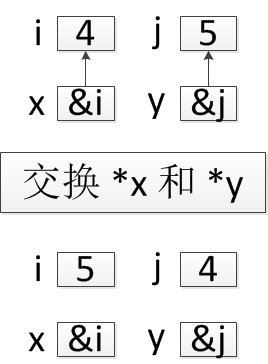
\includegraphics[width=0.6\textwidth]{exp5-3-1-2-a}
\end{figure}

\end{itemize}
\end{columns}

\end{frame}


\begin{frame}[fragile]
    {5.3.1 参数传递\small{~---~值传递}}
        \begin{block}{地址传递}
将实参的地址传递给形参,也就是说形参的类型为指针类型,通过形参改变实参的值。
\end{block}
\begin{columns}
\column{0.45\textwidth}
\begin{blueblock}<2->{示例2}\vspace{-3.5mm}\begin{lstlisting}
void Swap(int *x, int *y) {
    int *z(x);
    x = y;
    y = z;
}
int main() {
    int i(4), j(5);
    Swap(&i, &j);
    cout << "i=" << i << ",j=" << j << endl;
    return 0;
}
\end{lstlisting}\vspace{-1.5mm}
\end{blueblock}
\column{0.45\textwidth}
\begin{itemize}
  \item<3->[]

\begin{figure}
  \centering
  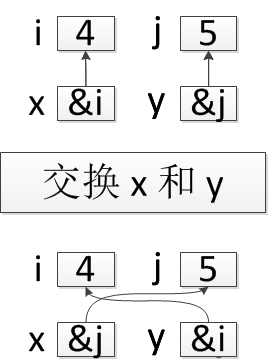
\includegraphics[width=0.6\textwidth]{exp5-3-1-2-b}
\end{figure}

\end{itemize}
\end{columns}

\end{frame}


\subsection{引用传递}\label{chap5-3-2}
\begin{frame}[fragile]
    {5.3 参数传递\small{~---~引用传递}}
\begin{block}{引用传递}
形参是实参的引用
\begin{itemize}
  \item 引用类型;
  \item 通过形参改变实参的值。
\end{itemize}
\end{block}
\begin{blueblock}<2->{引用传递的例子}\vspace{-1.5mm}\begin{lstlisting}
void Swap(int &x, int &y) {//x和y分别是实参i和j的别名
    int z(x);
    x = y;
    y = z;
} //交换x和y所绑定的对象的值
int main() {
    int i(4), j(5);
    Swap(i, j);
    cout << "i=" << i << ",j=" << j << endl;//输出i=5,j=4
    return 0;
}
\end{lstlisting}\vspace{-1.5mm}
\end{blueblock}

\end{frame}



\subsection{const~形参}

\begin{frame}[fragile]
    {5.3.3 参数传递\small{~---~const~形参}}
\begin{block}{const~形参}
~const~修饰的形参名字和~const~修饰的对象名字的含义相同。
\end{block}
\begin{blueblock}<2->{请问以下~const~修饰的形参名字的含义}\vspace{-1.5mm}\begin{lstlisting}
void f_cval(const int i);
void f_cptr(const int *i);
void f_cref(const int &i);
\end{lstlisting}\vspace{-1.5mm}
\end{blueblock}

\end{frame}
\begin{frame}[fragile]
    {5.3.3 参数传递\small{~---~const~形参}}
\begin{block}{const~形参}
~const~修饰的形参名字和~const~修饰的对象名字的含义相同。
\end{block}
\begin{blueblock}{请问以下~const~修饰的形参名字的含义}\vspace{-1.5mm}\begin{lstlisting}
void f_cval(const int i); //i 为 const 对象
void f_cptr(const int *i);//i 指向 const 类型的实参
void f_cref(const int &i);//i 为 const 类型实参的引用
\end{lstlisting}\vspace{-1.5mm}
\end{blueblock}

\end{frame}


\begin{frame}[fragile]
    {5.3.3 参数传递\small{~---~const~形参}}
\begin{block}{兼顾效率与安全}
\begin{itemize}
  \item 避免内容的拷贝:高效性;
  \item 不能通过形参改变实参:安全性。
\end{itemize}
\end{block}
\begin{blueblock}<2->{const~引用形参可以接受字面值常量、表达式的求值结果、需要转换的对象或者~const~对象,但引用形参是不可以的。}\vspace{-1.5mm}\begin{lstlisting}
void f_ref(int &i);//引用形参
const int cx = 1;
int x = 1;
f_ref(41);//错误:左值引用不能绑定字面值常量
f_ref(cx);//错误:左值引用不能绑定常量
f_ref(x+1);//错误:左值引用不能绑定右值表达式
\end{lstlisting}\vspace{-1.5mm}
\end{blueblock}
\begin{redblock}<3->{建议}
尽量使用引用形参,需要的时候使用指针形参
\end{redblock}
\end{frame}


\subsection{数组形参}
\begin{frame}[fragile]
    {5.3 参数传递\small{~---~数组形参}}
\begin{columns}
\column{0.45\textwidth}
\begin{block}{数组的特点}
\begin{itemize}
  \item 不可复制;
  \item 指针化。
\end{itemize}
\end{block}
\column{0.45\textwidth}
\begin{block}<2->{数组形参}
通常使用指针的方式来传递首元素的地址。
\end{block}
\end{columns}
\begin{blueblock}<3->{示例}\vspace{-1.5mm}\begin{lstlisting}
void fun(int *p);
void fun2(int p[]);//等价于上式,数组的方式
\end{lstlisting}\vspace{-1.5mm}
\end{blueblock}
\begin{blueblock}<4->{调用方式}\vspace{-1.5mm}\begin{lstlisting}
int arr[5] = {1, 2};
fun(arr); //正确:数组名转化为首元素的地址
fun(&arr[0]);//正确:显式传递首元素的地址
\end{lstlisting}\vspace{-1.5mm}
\end{blueblock}

\begin{redblock}<5->{传递的是数组首元素的地址,编译器不会检查数组的大小}
\vspace{-1.5mm}\begin{lstlisting}
void fun(int p[5]); //“指明”数组的长度,无用
\end{lstlisting}\vspace{-1.5mm}
\end{redblock}
\end{frame}


\begin{frame}[fragile]
    {5.3.3 参数传递\small{~---~数组形参}}
\begin{blueblock}<1->{显式传递数组的长度}\vspace{-2.5mm}\begin{lstlisting}
void print(char *str, unsigned size) {
    for (unsigned i = 0; i < size; ++i)
        cout << str[i];
}
\end{lstlisting}
\vspace{-1.5mm}
\end{blueblock}
%\vspace{-2em}
\begin{columns}
\column{0.48\textwidth}
\begin{blueblock}<2->{使用标记位来识别数组长度}\vspace{-1.5mm}\begin{lstlisting}
void print(char *str) {
    if (str) //如果str不是一个空指针
        while (*str) //当前指针指向非空字符
            cout << *str++; //输出当前指针指向的字符并指向下一个字符
}
    char arr[] = "Hello C++";
    print(arr);
\end{lstlisting}\vspace{-1.5mm}
常处理~C~风格的字符数组,对其他数据类型的数组可能没有效果。
\end{blueblock}
\column{0.48\textwidth}
\begin{blueblock}<3->{利用指针标明访问范围}\vspace{-1.5mm}\begin{lstlisting}
void print(char *beg, char * end) {
    //输出beg和end之间的元素(包含beg但不包含end指向的元素)
    while (beg != end)
         cout << *beg++; //输出当前指针指向的字符并指向下一个字符
}
    char arr[] = "Hello C++";
    print(begin(arr), end(arr));
\end{lstlisting}\vspace{-1.5mm}
~begin~和~end~函数可以获取数组的首元素和尾后元素的地址。
\end{blueblock}
\end{columns}
\end{frame}


\begin{frame}[fragile]
    {5.3.3 参数传递\small{~---~数组形参}}

\begin{blueblock}<1->{使用~const~形参}\vspace{-2.5mm}\begin{lstlisting}
void print(const char *str);
void print(const char *str, unsigned size);
void print(const char *beg, const char * end);
\end{lstlisting}\vspace{-1.5mm}
\end{blueblock}
\begin{block}<2->{使用~const~形参提高安全性}
只有当对数组进行写操作时,数组形参才使用非~const~类型,否则一律要使用~const~修饰,保证程序的安全性。
\end{block}
\begin{yellowblock}<3->{课下思考}
如何传递一个数组而非首元素地址?并分析以这种参数传递方式编写的函数是否可以处理任意长度的数组。

\end{yellowblock}

\end{frame}


\begin{frame}[fragile]
    {5.3.3 参数传递\small{~---~数组形参}}
\begin{block}{多维数组特点}
\begin{itemize}
  \item 传递的是数组的首元素地址;
  \item 编译器只忽略第一维的长度。
\end{itemize}
\end{block}
\begin{blueblock}<2->{使用~const~形参示例}\vspace{-2.5mm}\begin{lstlisting}
void fun(int (*a2d)[5]);  //a2d 指向一个含有5个元素的一维实参数组
void fun(int a2d[][5]);  //与上式等价
int matrix[4][5] = {};
fun(matrix); //传递 matrix 首元素地址,即一个具有5个元素的一维数组
\end{lstlisting}
\end{blueblock}

\end{frame}

%#####################################
\section{返回值类型}

\begin{frame}[fragile]
    {5.4 返回值类型}
\begin{block}{返回值类型}
\begin{itemize}
  \item 有值返回;
  \item 无值返回(返回一个~void~类型)。
\end{itemize}
\end{block}
\end{frame}


\begin{frame}[fragile]
    {5.4 返回值类型\small{~---~无值返回}}
\begin{blueblock}<1->{无值返回示例}
\vspace{-2.5mm}\begin{lstlisting}
void Swap(int &x, int &y) {
    if (x == y)
        return;
    int z(x);
    x = y;
    y = z;
}
\end{lstlisting}\vspace{-1.5mm}
\end{blueblock}
\begin{greenblock}{问题}
~return~的作用是什么?
\end{greenblock}
\end{frame}


\begin{frame}[fragile]
    {5.4 返回值类型\small{~---~无值返回}}
\begin{blueblock}<1->{无值返回示例}
\vspace{-2.5mm}\begin{lstlisting}
void Swap(int &x, int &y) {
    if (x == y)
        return;//显式返回主调函数
    int z(x);
    x = y;
    y = z;
    //隐式返回主调函数,无需return语句
}
\end{lstlisting}\vspace{-1.5mm}
\end{blueblock}
\begin{greenblock}{回答}
使用~return~语句来控制程序执行的流向。
\end{greenblock}
\end{frame}


\begin{frame}[fragile]
    {5.4 返回值类型\small{~---~有值返回}}
\begin{block}{有值返回}
\begin{itemize}
  \item 值返回(return by value\index{R!return by value});
  \item 引用返回(return by reference\index{R!return by reference});
  \item 指针返回(return by pointer\index{R!return by pointer})。
\end{itemize}
\end{block}
\end{frame}



\begin{frame}[fragile]
    {5.4.2 返回值类型\small{~---~有值返回}}
\begin{block}{值返回}
通过拷贝返回值的方式将结果传递给主调函数。
\begin{itemize}
  \item 简单;
  \item 安全;
  \item 效率低。
\end{itemize}
\end{block}
\begin{blueblock}<2->{值返回示例}
\vspace{-2.5mm}\begin{lstlisting}
int maximum(int a, int b) {
    return a > b ? a : b;
}
\end{lstlisting}\vspace{-1.5mm}
\end{blueblock}

\begin{greenblock}<3->{问题}
\begin{itemize}
  \item<3->[]为什么值返回效率低?

  \item<4->[]
\vspace{-3mm}\begin{lstlisting}
int a = 10, b = 5;
int c = maximum(a, b);
\end{lstlisting}\vspace{-1.5mm}
maximum~函数返回值存放在一个临时对象里,用来初始化对象~c。
\end{itemize}

\end{greenblock}

\end{frame}



\begin{frame}[fragile]
    {5.4.2 返回值类型\small{~---~有值返回}}

\begin{block}{引用返回}
返回的对象的一个别名,与返回对象指向同一个存储空间,不会产生临时对象。
\end{block}
%\column{0.45\textwidth}
\begin{blueblock}<2->{引用返回示例}
\vspace{-2.5mm}\begin{lstlisting}
const int & maximum(const int &a, const int &b) {
     return a > b ? a : b; //返回对象a或对象b的引用
}
\end{lstlisting}\vspace{-1.5mm}
调用~maximum~函数
\vspace{-2.5mm}\begin{lstlisting}
int x,y;
cin >> x >> y;
int z = maxinum(x,y);
\end{lstlisting}\vspace{-1.5mm}
\end{blueblock}
\begin{blueblock}<3->{定义x或y的引用}
\vspace{-2.5mm}\begin{lstlisting}
const int &ref = maximum(x,y);
\end{lstlisting}\vspace{-1.5mm}
\end{blueblock}
\end{frame}

\begin{frame}[fragile]
    {5.4.2 返回值类型\small{~---~有值返回}}
%\begin{columns}

%\column{0.45\textwidth}

\begin{columns}
\column{0.45\textwidth}
\begin{blueblock}<1->{返回一个非~const~左值引用}
\vspace{-2.5mm}\begin{lstlisting}
int& setMaximum(int &a, int &b) {
    //返回对象a 或对象b 的引用
    return a > b ? a : b;
}
int main(){
   int x = 0, y = 1;
   //把整数10赋值给 x 和 y 中较大者
   setMaximum(x, y) = 10;
   return 0;
}
\end{lstlisting}\vspace{-1.5mm}
\end{blueblock}
%\end{columns}
\column{0.45\textwidth}
\begin{blueblock}<2->{返回实参对象的地址}
\vspace{-2.5mm}\begin{lstlisting}
int* setMaximum(int &a, int &b) {
//返回引用a或b所绑定的实参对象的地址
    return a > b ? &a : &b;
}
int main(){
   int x = 0, y = 1;
   //通过返回指针把10赋值给 x和 y中较大者
   *setMaximum(x, y) = 10;
}
\end{lstlisting}\vspace{-1.5mm}
\end{blueblock}
\end{columns}
\end{frame}


\begin{frame}[fragile]
    {5.4.2 返回值类型\small{~---~有值返回}}
\begin{greenblock}{问题:下面程序是否有问题,为什么?如果有问题,该如何修改?}
\vspace{-2.5mm}\begin{lstlisting}
int& maximum(int a, int b) {
    return a > b ? a : b;
}
\end{lstlisting}\vspace{-1.5mm}
\end{greenblock}
\begin{greenblock}<2->{回答:切忌返回局部对象的地址或引用}
形参对象~a~和~b~都是局部对象,~maximum~函数终止时将会从内存中消亡,因此返回一个已经不存在的对象的引用是无效的引用。
\vspace{-2.5mm}\begin{lstlisting}
int& maximum(int a, int b) {
    static int c;
    c = a > b ? a : b;
    return c; //正确:返回静态局部对象c的引用
}
\end{lstlisting}\vspace{-1.5mm}
\end{greenblock}
\end{frame}


\begin{frame}[fragile]
    {5.4.2 返回值类型\small{~---~有值返回}}
\begin{block}{值返回方法比较}
\begin{itemize}
  \item 值返回方式可以返回局部对象的值,但需要借助于一个额外的临时对象完成值的返回;
  \item 引用和指针返回不需要借助于临时对象,但不能返回局部对象的引用或地址;
  \item 指针返回还经常用于返回一个具有动态存储周期的对象的地址。
\end{itemize}
根据实际需要并结合安全性和效率来进行选择
\end{block}

\end{frame}


%#####################################
\section{函数重载和特殊用途的函数}
\subsection{函数重载}\label{chap5-1-1}

\begin{frame}[fragile]
    {5.5 函数重载和特殊用途的函数\small{~---~函数重载}}
\begin{block}{重载}
把同一作用域下具有相同名字但不同形参列表的一组函数称为重载(overloaded\index{O!overloaded function})函数,这些函数执行相似的操作。
\end{block}
\begin{columns}
\column{0.45\textwidth}
\begin{blueblock}<2->{示例}
\vspace{-2.5mm}\begin{lstlisting}
const int& getMax(const int &a, const int &b) {
    return a > b ? a : b;
}
const int& getMax(const int &a, const int &b, const int &c) {
    return a > b ? (a > c ? a : c) : (b > c ? b : c);
}
const string& getMax(const string &a, const string &b) {
    return a > b ? a : b;
}
\end{lstlisting}\vspace{-1.5mm}
\end{blueblock}
\column{0.45\textwidth}
\begin{block}<3->{最佳匹配的原则}
\begin{itemize}
  \item 如果有精确匹配的函数,则调用此函数;否则选择实参与形参类型最接近的转换函数;
  \item 如果有一个以上无法区分的匹配,则会出现二义性调用(ambiguous call\index{A!ambiguous call})错误;
  \item 如果找不到任何一个与实参相匹配的函数,则会出现无匹配错误。
\end{itemize}
\end{block}
\end{columns}
\end{frame}


\begin{frame}[fragile]
    {5.5 函数重载和特殊用途的函数\small{~---~函数重载}}
\begin{blueblock}<1->{示例}
\vspace{-2.5mm}\begin{lstlisting}
const int& getMax(const int &a, const int &b) {
    return a > b ? a : b;
}
const int& getMax(const int &a, const int &b, const int &c) {
    return a > b ? (a > c ? a : c) : (b > c ? b : c);
}
const string& getMax(const string &a, const string &b) {
    return a > b ? a : b;
}
\end{lstlisting}\vspace{-1.5mm}
\end{blueblock}

\begin{greenblock}<2->{问题:以下函数调用第几个重载函数?}
\vspace{-2.5mm}\begin{lstlisting}
getMax(7, 8);
getMax("C++", "Programming");
\end{lstlisting}\vspace{-1.5mm}
\end{greenblock}
\end{frame}


\subsection{默认参数}\label{chap5-5-2}
\begin{frame}[fragile]
    {5.5 函数重载和特殊用途的函数\small{~---~默认参数}}
    \begin{block}{默认参数}
函数的某些形参总是接受一个默认的实参值(default argument\index{D!default argument})。
\end{block}
\begin{columns}
\column{0.45\textwidth}
\begin{blueblock}<2->{示例}
\vspace{-2.5mm}\begin{lstlisting}
void turnoff(int time = 21);
\end{lstlisting}\vspace{-1.5mm}
\end{blueblock}
\column{0.45\textwidth}
\begin{blueblock}<3->{使用}
\vspace{-2.5mm}\begin{lstlisting}
turnoff(); //省略实参,使用默认值
turnoff(22); //提供实参,接受实参值
\end{lstlisting}\vspace{-1.5mm}
\end{blueblock}
\end{columns}
\begin{blueblock}<4->{形参的默认值可以是任何可以转换成形参类型的表达式}
\vspace{-2.5mm}\begin{lstlisting}
void turnoff(int time = getTime());
\end{lstlisting}\vspace{-1.5mm}
\end{blueblock}
\end{frame}

\begin{frame}[fragile]
    {5.5.2 函数重载和特殊用途的函数\small{~---~默认参数}}
    \begin{block}{具有多个默认值}
一个函数可以有多个默认值,但所有具有默认值的参数必须\alert{靠右侧}放置。
\end{block}
\begin{greenblock}<2->{定义是否正确?}
\vspace{-2.5mm}\begin{lstlisting}
void print(int a, int b, int c = 3);
void print(int a, int b = 2, int c);
void print(int a = 1, int b = 2, int c = 3);
\end{lstlisting}\vspace{-1.5mm}
\end{greenblock}

\begin{greenblock}<3->{答案}
\vspace{-2.5mm}\begin{lstlisting}
void print(int a, int b, int c = 3); //正确:部分参数具有默认值
void print(int a, int b = 2, int c); //错误:最右侧参数没有默认值
void print(int a = 1, int b = 2, int c = 3); //正确:所有参数具有默认值
\end{lstlisting}\vspace{-1.5mm}
\end{greenblock}
\end{frame}





\subsection{内联函数}
\begin{frame}[fragile]
    {5.5 函数重载和特殊用途的函数\small{~---~内联函数}}
    \begin{block}{函数优缺点}
\begin{itemize}
  \item 函数的使用体现了模块化程序设计思想,降低了程序设计的复杂性;
  \item 函数调用,比如执行流的转移操作、参数传递、返回值处理等,需要时间和空间的开销。
\end{itemize}
C++~提供了一种即保证函数化的形式又兼顾执行效率的方法:\alert{内联函数}。
\end{block}
\begin{blueblock}<2->{示例}
\vspace{-2.5mm}\begin{lstlisting}
inline void Swap(int &x, int &y){ /*...*/ }
\end{lstlisting}\vspace{-1.5mm}
\end{blueblock}
\begin{block}<3->{减少开销}
编译器将在调用处嵌入内联函数的代码,不会发生函数调用,因而也不会产生函数调用的开销了。
\end{block}
\begin{redblock}<4->{注意}
对于编译器来说,inline~关键字只是一个建议。
\end{redblock}
\end{frame}

\begin{frame}[fragile]
    {5.5 函数重载和特殊用途的函数\small{~---~内联函数}}
\begin{greenblock}{例 5.2}
利用冒泡排序法将容器中的学生成绩排序。
\end{greenblock}
\begin{itemize}
  \item<2->[]
\begin{figure}
  \centering
  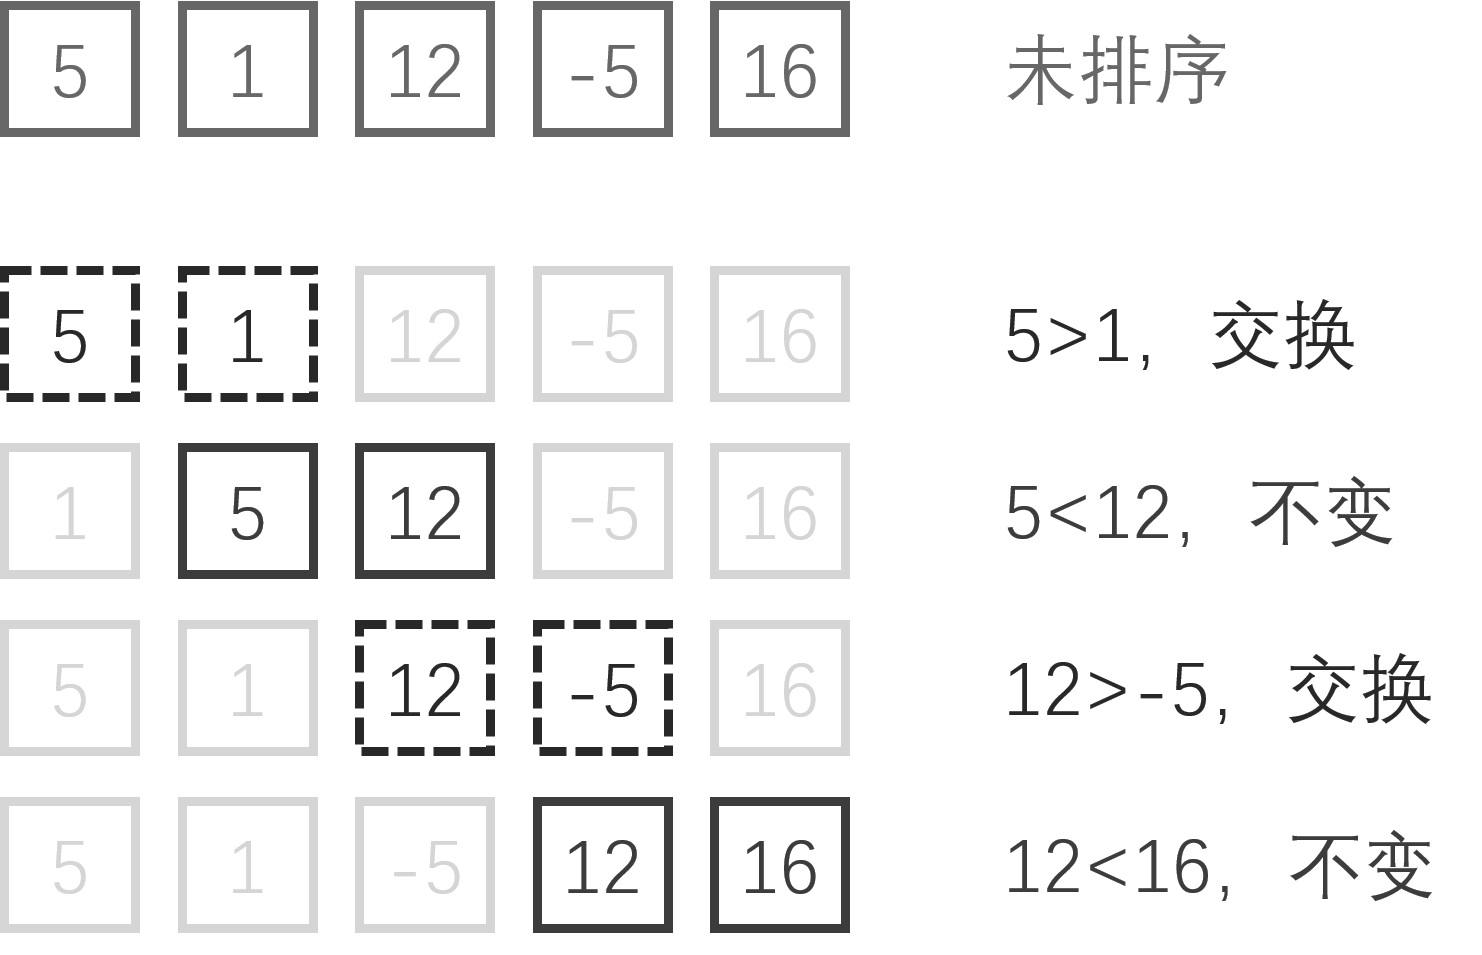
\includegraphics[width=0.7\textwidth]{Fig7-3}
\end{figure}

\end{itemize}
\end{frame}




\begin{frame}[fragile]
    {5.5 函数重载和特殊用途的函数\small{~---~内联函数}}
\vspace{-1em}
\begin{blueblock}{利用冒泡排序法将容器中的学生成绩排序}
\vspace{-3.5mm}\begin{lstlisting}
inline void Swap(int &x, int &y) {
    int z(x);
    x = y;
    y = z;
}
int main() {
    srand(0);
    vector<int> score(10);
    for (auto &i : score)
        i = rand() % 100;
    for (int i = score.size()-1; i >=0; --i) {
        for (int j = 0; j < i;++j) {//每一轮冒泡过程将最大的数浮出来(右边)
             if (score[j+1] < score[j])//相邻的两个数比较
                 Swap(score[j+1], score[j]);
        }
    }
    for (auto &i : score)
        cout << i << endl;
    return 0;
}
\end{lstlisting}\vspace{-1.5mm}
\end{blueblock}
\end{frame}


%--------------------


\subsection{constexpr~函数*}
\begin{frame}[fragile]
    {5.5 函数重载和特殊用途的函数\small{~---~constexpr~函数*}}

    \begin{greenblock}{问题}
    \begin{itemize}
      \item<1->[]
      以下程序是否正确,为什么,该如何修改?
\vspace{-2.5mm}\begin{lstlisting}
const int getNumber() { return 10; }
const int numStudent = getNumber();

int arr[numStudent];
\end{lstlisting}\vspace{-1.5mm}
      \item<2->[]
      此时编译器会报错,提示无法在编译时计算~numStudent~的值。这是因为只能在运行期间调用函数~getNumber~后才能计算~numStudent~的值。
    \end{itemize}
    \end{greenblock}

\end{frame}


\begin{frame}[fragile]
    {5.5 函数重载和特殊用途的函数\small{~---~constexpr~函数*}}

\begin{block}<1->{constexpr~函数}
constexpr~函数指的是能用于常量表达式的函数。要求:
\begin{itemize}
  \item 函数体中有且仅有一条~return~语句;
  \item 函数返回值类型不能为~void;
  \item return~语句中的表达式必须是编译时的常量表达式。
\end{itemize}

\end{block}
\begin{blueblock}<2->{示例}
\vspace{-2.5mm}\begin{lstlisting}
constexpr int f() { return 10; }
constexpr int getNumber(int i) { return i; }
int stu1[getNumber(10)]; //正确:getNumber(10)是常量表达式
int num = 10;
int stu2[getNumber(num)]; //错误:运行时才能确定num的值
\end{lstlisting}\vspace{-1.5mm}
\end{blueblock}
\begin{redblock}<3->{提示}
constexpr~函数会隐式转化为内联函数。
\end{redblock}
\end{frame}




%#####################################
\section{函数指针和~lambda~表达式}
\subsection{函数指针}\label{chap5-6-1}
\begin{frame}[fragile]
    {5.6 函数指针和~lambda~表达式\small{~---~函数指针}}

\begin{block}{函数指针}
\begin{itemize}
  \item 函数名对应于函数的执行代码的入口地址;
  \item 指针可以指向一个函数;
  \item 函数的类型由\alert{返回值类型}和\alert{形参列表}决定。
\end{itemize}
\end{block}

\begin{blueblock}<2->{示例}
\vspace{-2.5mm}\begin{lstlisting}
//声明一个~compareInt~函数:比较两个整数大小
bool compareInt(int, int);
bool(*pf)(int, int);//定义一个指向此类型函数的指针
\end{lstlisting}\vspace{-1.5mm}
\end{blueblock}


\begin{greenblock}<3->{问题:请说明下面指针的含义?}

\begin{itemize}
\item<3->[]
\vspace{-2.5mm}\begin{lstlisting}
bool* pf(int, int);
\end{lstlisting}\vspace{-1.5mm}
\item<4->[]
函数名为~pf,返回值类型为~bool*~的函数声明。
\end{itemize}
\end{greenblock}

\end{frame}


\begin{frame}[fragile]
    {5.6.1 函数指针和~lambda~表达式\small{~---~函数指针}}
    \begin{block}{简化函数指针定义}
利用类型别名关键字~typedef\index{T!typedef}~或~using~来简化函数指针的定义。
\end{block}

\begin{blueblock}<2->{示例}
\vspace{-2.5mm}\begin{lstlisting}
typedef bool(*pFun)(int, int);
using pFun = bool(*)(int, int);//与上式等价

pFun pf; //和定义普通指针一样的方式来定义一个函数指针
\end{lstlisting}\vspace{-1.5mm}
\end{blueblock}
\end{frame}


\begin{frame}[fragile]
    {5.6.1 函数指针和~lambda~表达式\small{~---~函数指针}}
    \begin{block}{函数指针初始化}
和普通指针类型一样,应该在定义函数指针时初始化
\end{block}

\begin{blueblock}<2->{示例}
\vspace{-2.5mm}\begin{lstlisting}
pFun pf1 = compareInt; //隐式初始化,pf1指向compareInt函数
pFun pf2 = &compareInt; //显式初始化,pf2指向compareInt函数
pFun pf3 = nullptr; //pf3不指向任何函数
\end{lstlisting}\vspace{-1.5mm}
\end{blueblock}

\begin{blueblock}<3->{示例}
当一个指针指向了一个具体的函数后,可以通过该指针来调用其指向的函数
\begin{lstlisting}
bool b1 = pf1(1, 2);
bool b2 = (*pf2)(1, 2);
\end{lstlisting}\vspace{-1.5mm}
\end{blueblock}
\end{frame}




\begin{frame}[fragile]
    {5.6.1 函数指针和~lambda~表达式\small{~---~函数指针}}

\begin{greenblock}{例 5.3}
利用梯形法设计一个求数值积分的通用函数。
\end{greenblock}
\begin{yellowblock}<2->{提示}
想要实现一个求积分的通用函数,可以将待求积分函数以参数的形式传递到这个通用函数里面,然后利用梯形法求解被积函数的积分。
\end{yellowblock}
\begin{itemize}
  \item[]<3->
            \begin{figure}[ht]
                \centering
                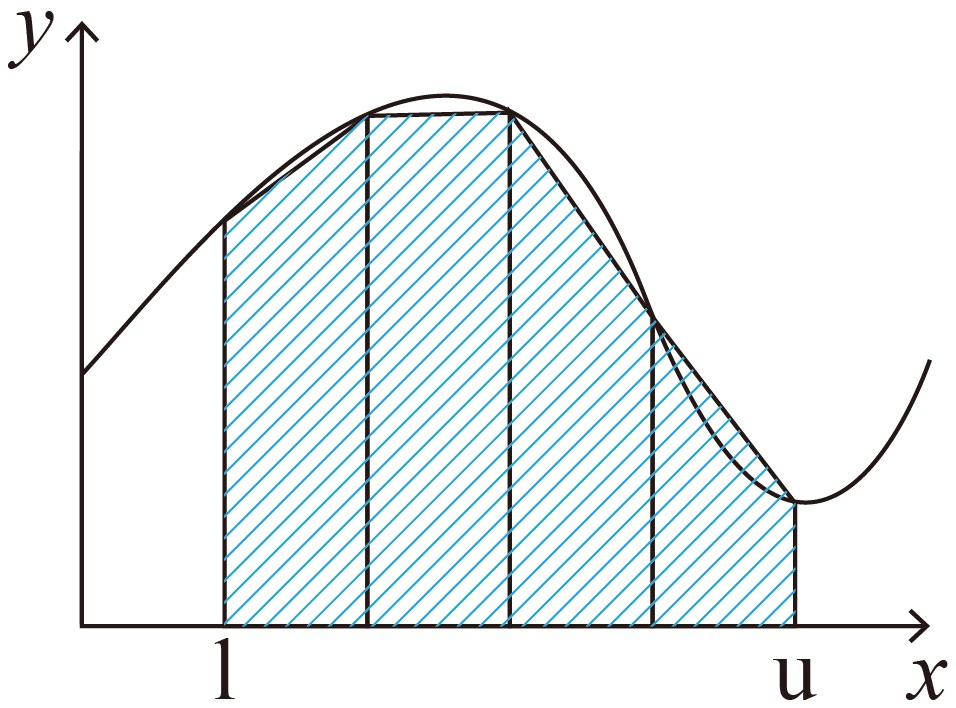
\includegraphics[width=0.4\textwidth]{Fig5-2}
                \caption{梯形法求积分示例图}
                % \label{fig:label}
            \end{figure}
\end{itemize}
\end{frame}


\begin{frame}[fragile]
    {5.6.1 函数指针和~lambda~表达式\small{~---~函数指针}}
\vspace{-0.5em}
\begin{blueblock}{代码清单5.3,例 5.3}
\vspace{-2.5mm}\begin{lstlisting}
using pFun = double(*)(double);
double f_sphere(double x) {
    return x*x;
}
double f_default(double x) {
    return 0;
}
double f_sin(double x) {
    return sin(x);
}
double integrate(double l, double u, pFun pf = f_default, int n = 1000) {
    double sum = 0.0;
    double gap = (u - l) / n;  //每个间隔的长度
    for (int i = 0; i < n; i++)
        sum += (gap / 2.0) * (pf(l + i*gap) + pf(l + (i + 1)*gap));
    return sum;
}
int main() {
    cout<<"默认函数在区间[0:1]上的积分为:"<<integrate(0, 1) << endl;
    cout<<"Sphere函数在区间[0:1]上的积分为:"<<integrate(0, 1, f_sphere)<<endl;
    cout<<"sin函数在区间[0:1]上的积分为:"<<integrate(0, 1, f_sin)<<endl;
}
\end{lstlisting}\vspace{-1.5mm}
\end{blueblock}
\end{frame}


\begin{frame}[fragile]
    {5.6.1 函数指针和~lambda~表达式 \small{~---~函数指针}}
    \begin{block}{识别指针的原则}
\begin{itemize}
  \item 取出标识符;
  \item 由里向外;
  \item 由右向左。
\end{itemize}
\end{block}

\begin{columns}
\column{0.45\textwidth}
\begin{blueblock}<2->{简单例子}
\vspace{-2.5mm}\begin{lstlisting}
int(*p1)[5];
int *p2[5];
int *&p3 = p2[0];
\end{lstlisting}\vspace{-1.5mm}
\end{blueblock}
\column{0.45\textwidth}
\begin{blueblock}<3->{识别指针}
\vspace{-2.5mm}\begin{lstlisting}
void(*a[5])(int);
void(*(*b)[5])(int);
void(*c(int, void(*fp)(int)))(int);
\end{lstlisting}\vspace{-1.5mm}
\end{blueblock}
\end{columns}

\begin{blueblock}<4->{利用~using~声明简化语句}
\begin{lstlisting}
using PF = void(*)(int);
PF *a[5];
PF(*b)[5];
PF c(int, PF);
\end{lstlisting}\vspace{-1.5mm}
\end{blueblock}


\end{frame}

\subsection{lambda~表达式}\label{chap5-6-2}
\begin{frame}[fragile]
    {5.6 函数指针和~lambda~表达式\small{~---~lambda~表达式}}

    \begin{block}{~lambda~表达式}
\begin{itemize}
  \item 只使用一次;
  \item 临时的匿名函数,表示一个可以调用的代码单元;
  \item 与函数类似,lambda~表达式具有返回值、形参列表和函数体;
  \item 可定义在一个函数内部。
\end{itemize}
\end{block}

\begin{block}<2->{1.~定义~lambda~表达式}
\centering [captures](parameters) -> return type \{statements\}\\
\begin{itemize}
  \item captures:指定在同一作用域下~lambda~主体捕获(访问)哪些对象以及如何捕获这些对象;
  \item parameters:形参列表;
  \item return type:返回值类型;
  \item statements:函数体。
\end{itemize}
\end{block}

\end{frame}

\begin{frame}[fragile]
    {5.6 函数指针和~lambda~表达式\small{~---~lambda~表达式}}


\begin{blueblock}<1->{~auto~关键字}
\begin{lstlisting}
auto fun = [](int i) {cout << i << endl; };
fun(17); //输出17
\end{lstlisting}
\begin{itemize}
  \item ~auto~关键字把一个~lambda~表达式存放到一个对象
  \item lambda~可以根据函数主体来推断返回类型。
\end{itemize}
\end{blueblock}

\begin{blueblock}<2->{显式指明~return type}
\begin{lstlisting}
[](int i)->int { return i*i; }
\end{lstlisting}
\end{blueblock}

\end{frame}

\begin{frame}[fragile]
    {5.6.2 函数指针和~lambda~表达式\small{~---~捕获对象}}
    \begin{block}{捕获对象}
lambda~可以捕获外围作用域内的局部对象,而且还可以指定捕获的方式
\end{block}
\begin{columns}
\column{0.45\textwidth}
\begin{blueblock}<2->{按值捕获特定的外围对象}
\vspace{-2.5mm}\begin{lstlisting}
int divisor = 5;
vector<int> numbers{ 1, 2, 3, 4, 5, 10, 15, 20, 25, 35, 45, 50 };
for_each(numbers.begin(), numbers.end(), [divisor](int y) {
    //divisor为外围divisor的拷贝
    if (y % divisor == 0)
        cout << y << endl;
    //输出被divisor整除的元素
});
\end{lstlisting}\vspace{-1.5mm}
divisor 作为副本在函数体内部使用
\end{blueblock}
\column{0.45\textwidth}
\begin{blueblock}<3->{按引用捕获特定的外围对象}
\vspace{-2.5mm}\begin{lstlisting}
int sum = 0;

for_each(numbers.begin(), numbers.end(), [divisor, &sum](int y) {
    //sum为外围sum 的引用
    if (y % divisor == 0)
        sum += y;
    //累加被divisor整除的元素,结果存放到外围对象sum中
});

\end{lstlisting}\vspace{-1.5mm}
sum 作为引用在函数体内部使用
\end{blueblock}
\end{columns}
\begin{blueblock}<4->{按引用捕获特定的外围对象}
\text{[=]}和[\&]分别以值捕获和引用捕获方式捕获外围所有对象
\end{blueblock}
\end{frame}


%#####################################
\section{递归调用}
\begin{frame}[fragile]
    {5.7 递归调用}
    \begin{block}{递归调用}
一个函数直接或间接地调用自己,这个函数称为递归函数(recursive function\index{R!recursive function})
\begin{itemize}
  \item 易实现;
  \item 可读性强。
\end{itemize}
\end{block}
\end{frame}


\subsection{递推和回归}
\begin{frame}[fragile]
    {5.7 递归调用\small{~---~递推和回归}}
\begin{greenblock}{例 5.4}
求解以下数列的第~n~项。\label{exam5-4}
\[f(n)=
 \begin{cases}
    0       & \quad  n=0\\
    f(n-1)+n  & \quad n>0\\
  \end{cases}
  \]
\end{greenblock}

\end{frame}


\begin{frame}[fragile]
    {5.7 递归调用\small{~---~递推和回归}}
\begin{columns}
\column{0.45\textwidth}
\begin{blueblock}<1->{例 5.4}
\vspace{-2.5mm}\begin{lstlisting}
#include<iostream>
int sumTo(int i) {
    if (i == 0)  return 0;
    return  sumTo(i - 1) + i;
}
int main() {
    std::cout << sumTo(3);
    return 0;
}
\end{lstlisting}\vspace{-1.5mm}
\end{blueblock}
\column{0.55\textwidth}

\begin{figure}[ht]
    \centering
    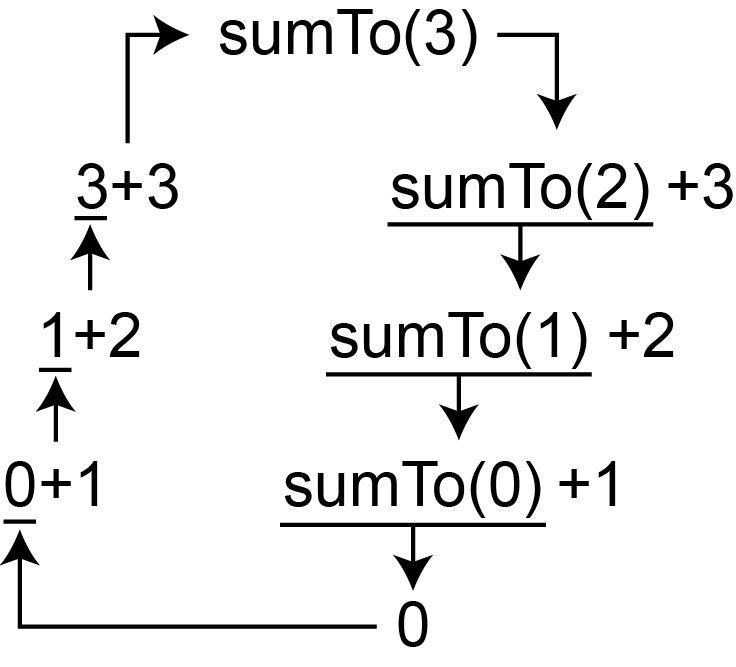
\includegraphics[width=0.5\textwidth]{Fig5-3}
     \caption{函数调用~sumTo(3)~的执行过程}
    % \label{fig:label}
\end{figure}
\end{columns}
    \begin{block}<2->{递归调用三要素}
\begin{itemize}
  \item 递推;
  \item 回归;
  \item 终止条件。
\end{itemize}
\end{block}
\end{frame}


\begin{frame}[fragile]
    {5.7 递归调用\small{~---~递推和回归}}

\begin{greenblock}{例 5.5}
汉诺塔问题(Tower of Hanoi)。如图所示,有~A、B、C~三个柱子,A~柱上有~n~个大小不同的盘子,大盘在下、小盘在上依次存放。要求将~A~柱上的盘子全部移动到~C~柱上,每一次只能移动一个盘子,可以借助任何一个柱子,但必须要保证在任意时刻大盘在下、小盘在上。
\end{greenblock}

\begin{itemize}
  \item<2->[]
  \begin{figure}[h]
\centering
 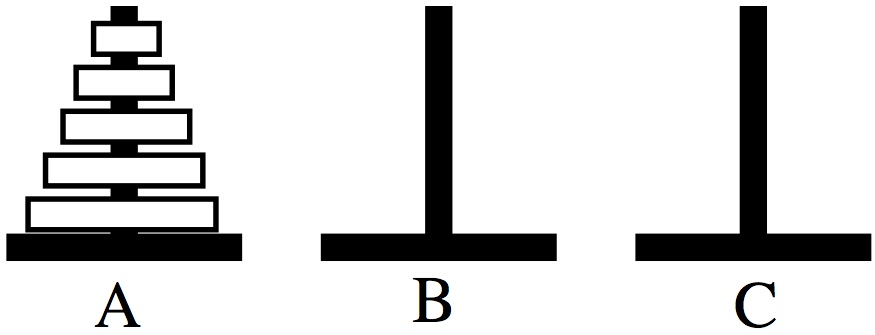
\includegraphics[width=0.5\textwidth]{Fig5-4}
\end{figure}
\end{itemize}

\end{frame}




\begin{frame}[fragile]
    {5.7 递归调用\small{~---~递推和回归}}

\begin{yellowblock}<1->{分析}
要想将~n~个盘子从~A~柱移到~C~柱,有三个步骤必须要完成:%1)先把~A~柱上~n-1~个盘子移到~B~柱上;2)将第~n~个盘子移到~C~柱上;3)将~n-1~个盘子从~B~ 柱移动~C~ 柱上。
\begin{itemize}
  \item 先把~A~柱上~n-1~个盘子移到~B~柱上;
  \item 将第~n~个盘子移到~C~柱上;
  \item 将~n-1~个盘子从~B~ 柱移动~C~ 柱上。
\end{itemize}
\end{yellowblock}
\begin{yellowblock}<2->{目标}
设计递归函数,其功能是将~n~个盘子从初始柱~src~上借助中间柱~mid~移动到目标柱~tar~上。
\end{yellowblock}

\end{frame}




\begin{frame}[fragile]
    {5.7 递归调用\small{~---~递推和回归}}
\begin{columns}
\column{0.55\textwidth}
\begin{blueblock}<1->{汉诺塔问题}
\vspace{-2.5mm}\begin{lstlisting}
#include<iostream>
using namespace std;
void hanoi(int n, char src, char mid, char tar) {
    if (n == 1)
        cout << src << "->" << tar << '\t';
    else {
        //将n-1个盘子移到中间柱上
        hanoi(n - 1, src, tar, mid);
        //将最后一个盘子移到目标柱上
        cout<<src<<"->"<< tar << '\t';
        //将n-1个盘子从中间柱移到目标柱上
        hanoi(n - 1, mid, src, tar);
    }
}
int main() {
    int n;
    cin >> n;
    hanoi(n, 'A', 'B', 'C');
    return 0;
}
\end{lstlisting}\vspace{-1.5mm}
\end{blueblock}
\column{0.45\textwidth}
\begin{itemize}
  \item<2->[]
  	\begin{figure}
		\centering
		\animategraphics[scale=0.2,autoplay,loop]{1}{exp5-7/exp5-7-1-}{1}{8}
        \caption{移动过程}
	\end{figure}
\end{itemize}
\end{columns}

\end{frame}


\subsection{递归和循环}
\begin{frame}[fragile]
    {5.7 递归调用\small{~---~递归和循环}}
\begin{block}{递归和循环}
\begin{itemize}
  \item 递归程序的递推和回归过程可以用循环结构来实现;
  \item 和循环结构相比,递归函数实现简单并且思路清晰,但缺点是需要消耗内存和其它的函数调用开销
\end{itemize}
\end{block}

\end{frame}


\begin{frame}[fragile]
    {5.7 递归调用\small{~---~递归和循环}}
\begin{greenblock}<1->{例 5.6}
利用递归程序设计方法求解八皇后问题,要求找出所有可能方案。
\end{greenblock}

\begin{yellowblock}<2->{分析}
对于八皇后问题,每一次递推在新一行安排一个皇后。有两种情形需要回归:
\begin{itemize}
  \item 当前行没有可行位置,则程序需要回归,即进行回溯操作;
  \item 当所有的皇后都已经成功摆放,需要回归寻找下一个可行的方案。
\end{itemize}
\end{yellowblock}

\end{frame}




\begin{frame}[fragile]
    {5.7 递归调用\small{~---~递归和循环}}
%\vspace{-1em}
\begin{blueblock}<1->{代码清单5.6,例5.6}
\vspace{-2.5mm}\begin{lstlisting}
bool isSafe(int i, const vector<int> &que) {
    for (int k = 0; k < i; ++k)
        if (que[k] == que[i] || (abs(que[i] - que[k]) == abs(i - k)))
        return false;
    return true;
}
void queen(int i, vector<int> &que, int &cnt) {
    if (i == 8) {
        cout << "方案" << ++cnt << ":";
        for (int k = 0; k < que.size(); ++k) cout << que[k];
        return;
    }
    for (int k = 0; k < que.size(); ++k) {
        que[i] = k;
        if (isSafe(i, que)) queen(i + 1, que, cnt); //如果安全,安排下一行皇后
    }
}
int main() {
    constexpr int sz = 8; int cnt(0);
    vector<int> que(sz);
    queen(0, que, cnt);
}
\end{lstlisting}\vspace{-1.5mm}
\end{blueblock}
\end{frame}

%#####################################
\section{编译预处理和多文件结构}

\begin{frame}[fragile]
    {5.8 编译预处理和多文件结构}
\begin{block}{预处理指令}
\begin{itemize}
  \item 由~\#~符号开头;
  \item 每条指令占一行;
  \item 通常放在文件的开始部分。
\end{itemize}
例如
\begin{itemize}
  \item 文件包含指令~\#include~;
  \item 宏定义;
  \item 条件编译指令。
\end{itemize}
\end{block}
\end{frame}

\subsection{宏定义}\label{chap5-8-1}
\begin{frame}[fragile]
    {5.8 编译预处理和多文件结构\small{~---~宏定义}}
\begin{block}{宏定义}
\begin{itemize}
  \item 宏定义指令为~\#define;
  \item 功能是定义一个标识符来代替一串字符,该标识符称为宏名;
  \item 分为带参和不带参两种。
\end{itemize}
\end{block}
\begin{columns}
\column{0.4\textwidth}
\begin{block}<2->{1.不带参宏定义}
 \indent \#define 宏名~~~~字符串常量\\
 \begin{lstlisting}
#define PI 3.14159
void testPI() {
    cout << 2 * PI << endl;
}
//用来编译希望执行的代码
#define DEBUG

\end{lstlisting}\vspace{-1.5mm}
\end{block}
\column{0.5\textwidth}
\begin{block}<3->{2.带参宏定义}
 \indent \#define   ~~宏名(参数表)~~字符串常量\\
\begin{lstlisting}
#define fun2(a,b) (a)*(b)
#define fun3(a,b) a*b
void testFun() {
    cout << fun2(1 + 2, 3 - 2) << endl;
    cout << fun3(1 + 2, 3 - 2) << endl;
}//(*@\alert{参数必须用小括号括起来}@*)
\end{lstlisting}\vspace{-1.5mm}
\end{block}

\end{columns}
\begin{redblock}<4->{建议}
尽量使用~const~对象和内联函数
\end{redblock}
\end{frame}



\begin{frame}[fragile]
    {5.8.1 编译预处理和多文件结构~---~宏定义\small{~---~使用特殊操作符}}
\begin{block}{特殊操作符}
可以使用一些特殊的操作符来实现特殊的功能
\end{block}
\begin{columns}
\column{0.47\textwidth}
\begin{block}<2->{~字符串化操作符\#~}
把语言符号转化成字符串,即将后面的宏参数进行字符串化操作。\\
\indent \#define str(a) \#a\\
 \begin{lstlisting}
#define str(a) #a
cout << str(test) << endl;
\end{lstlisting}\vspace{-1.5mm}
等价于
 \begin{lstlisting}
cout << "test" << endl;
\end{lstlisting}\vspace{-1.5mm}
\end{block}
\column{0.47\textwidth}
\begin{block}<3->{连接符~\#\#}
将两个语言符号连接为一个语言符号\\
\indent \#define glue(a,b) a\#\#b\\
 \begin{lstlisting}
#define glue(a,b) a##b
glue(c, out) << "test" << endl;
int glue(x, 1) = 1;
\end{lstlisting}\vspace{-1.5mm}
等价于
 \begin{lstlisting}
cout << "test" << endl;
int x1 = 1;
\end{lstlisting}\vspace{-1.5mm}
\end{block}
\end{columns}
\end{frame}


\subsection{条件编译}

\begin{frame}[fragile]
    {5.8 编译预处理和多文件结构\small{~---~条件编译}}
\begin{block}{条件编译}
\begin{itemize}
  \item 程序中的代码在满足一定条件下才会被编译;
  \item 编译的条件有两类:宏名和常量表达式;
  \item 条件编译指令包括:
\#ifdef、\#ifndef、\#undef、 \#if、\#else、\#endif~ 等。
\end{itemize}
\end{block}
\begin{columns}
\column{0.45\textwidth}
\begin{block}<2->{例子1}
 \begin{lstlisting}
#ifdef DEBUG
    cout << "x=" << x << endl;
#endif
\end{lstlisting}\vspace{-1.5mm}
如果定义了~DEBUG~宏,则上述~cout~语句将被编译,否则将被忽略。

\end{block}
\column{0.45\textwidth}
\begin{block}<3->{例子2}
 \begin{lstlisting}
#if 0
    cout << "此行代码永远也不会被编译" << endl;
#endif
\end{lstlisting}\vspace{-1.5mm}
常量表达式的值为~false~,上面的~cout~语句永远也不会被编译。
\end{block}
\end{columns}
\end{frame}


\subsection{多文件结构}\label{chap5-8-3}

\begin{frame}[fragile]
    {5.8 编译预处理和多文件结构\small{~---~多文件结构}}
\begin{block}{多文件结构}
编写一个较大的程序时,通常根据代码之间的耦合关系将它们放到不同的文件里面,进行单独的编写与编译,最终完成一个完整的程序。
\begin{itemize}
  \item 标识符的可见性:把标识符的声明放到头文件里面,实现名字共享;

  \item 头文件保护:~\#ifndef、\#define 、~\#endif~预编译指令或者\#pragma once宏;
  \item 头文件包含\begin{itemize}
               \item 函数的声明
               \item const~对象
               \item 全局对象的声明
               \item 内联函数
               \item constexpr~函数
               \item 类和模版的定义
             \end{itemize}
\end{itemize}
\end{block}
\end{frame}


\begin{frame}[fragile]
    {5.8 编译预处理和多文件结构\small{~---~多文件结构}}
\begin{columns}
\column{0.54\textwidth}
\begin{block}{myHeader.h}
\vspace{-2.5mm} \begin{lstlisting}
#ifndef MYHEADER_H
#define MYHEADER_H
const double pi = 3.1415926;  //const对象
int add(int, int);//函数声明
extern int g_sum;   //全局对象声明
inline bool isNumber(char ch) {//内联函数
    return ch >= '0'&&ch <= '9' ? 1 : 0;
}
constexpr int scale() {  //constexpr 函数
    return 10;
}
class myClass {  };  // 类定义
template<typename T>  // 函数模板
const T& getMax(const T &a, const T &b) {
    return a > b ? a : b;
}
#endif // !MYHEADER_H
\end{lstlisting}\vspace{-1.5mm}
\end{block}
\column{0.4\textwidth}

\begin{block}<1->{add.cpp}
\vspace{-2.5mm} \begin{lstlisting}
int g_sum = 10;
int add(int a, int b) {
    return a + b;
}
\end{lstlisting}\vspace{-1.5mm}
\end{block}

\begin{block}<1->{multi\_file.cpp}
\vspace{-1.5mm} \begin{lstlisting}
#include "myHeader.h"
#include <iostream>
using namespace std;
int main() {
    g_sum = add(4, 5);
    cout << g_sum << endl;
    return 0;
}
\end{lstlisting}\vspace{-1.5mm}
\end{block}


\end{columns}

\end{frame}

%---------------------------------------------------------------------------------------------
\begin{frame}[fragile]{课后作业}
\begin{columns}[t]
\column{0.8\textwidth}
\begin{block}{作业本}
 \begin{enumerate}
   \item 习题5.6、5.9和5.17
 \end{enumerate}
\end{block}

\begin{block}{上机练习}
 \begin{enumerate}
   \item 实验指导书:第五章
 \end{enumerate}
\end{block}
\end{columns}
\end{frame}

\begin{frame}[fragile]
	\frametitle{~~}
	\begin{center}
		\huge{本章结束}
	\end{center}
\end{frame}


\end{document}
